\documentclass[
  bibliography=totoc,     % Literatur im Inhaltsverzeichnis
  captions=tableheading,  % Tabellenüberschriften
  titlepage=firstiscover, % Titelseite ist Deckblatt
]{scrartcl}

% Paket float verbessern
\usepackage{scrhack}

% Warnung, falls nochmal kompiliert werden muss
\usepackage[aux]{rerunfilecheck}

% unverzichtbare Mathe-Befehle
\usepackage{amsmath}
% viele Mathe-Symbole
\usepackage{amssymb}
% Erweiterungen für amsmath
\usepackage{mathtools}

% Fonteinstellungen
\usepackage{fontspec}
% Latin Modern Fonts werden automatisch geladen
% Alternativ zum Beispiel:
%\setromanfont{Libertinus Serif}
%\setsansfont{Libertinus Sans}
%\setmonofont{Libertinus Mono}

% Wenn man andere Schriftarten gesetzt hat,
% sollte man das Seiten-Layout neu berechnen lassen
\recalctypearea{}

% deutsche Spracheinstellungen
\usepackage[main=ngerman]{babel}


\usepackage[
  math-style=ISO,    % ┐
  bold-style=ISO,    % │
  sans-style=italic, % │ ISO-Standard folgen
  nabla=upright,     % │
  partial=upright,   % ┘
  warnings-off={           % ┐
    mathtools-colon,       % │ unnötige Warnungen ausschalten
    mathtools-overbracket, % │
  },                       % ┘
]{unicode-math}

% traditionelle Fonts für Mathematik
\setmathfont{Latin Modern Math}
% Alternativ zum Beispiel:
%\setmathfont{Libertinus Math}

\setmathfont{XITS Math}[range={scr, bfscr}]
\setmathfont{XITS Math}[range={cal, bfcal}, StylisticSet=1]

% Zahlen und Einheiten
\usepackage[
  locale=DE,                   % deutsche Einstellungen
  separate-uncertainty=true,   % immer Fehler mit \pm
  per-mode=symbol-or-fraction, % / in inline math, fraction in display math
]{siunitx}

% chemische Formeln
\usepackage[
  version=4,
  math-greek=default, % ┐ mit unicode-math zusammenarbeiten
  text-greek=default, % ┘
]{mhchem}

% richtige Anführungszeichen
\usepackage[autostyle]{csquotes}

% schöne Brüche im Text
\usepackage{xfrac}

% Standardplatzierung für Floats einstellen
\usepackage{float}
\floatplacement{figure}{htbp}
\floatplacement{table}{htbp}

% Floats innerhalb einer Section halten
\usepackage[
  section, % Floats innerhalb der Section halten
  below,   % unterhalb der Section aber auf der selben Seite ist ok
]{placeins}

% Seite drehen für breite Tabellen: landscape Umgebung
\usepackage{pdflscape}

% Captions schöner machen.
\usepackage[
  labelfont=bf,        % Tabelle x: Abbildung y: ist jetzt fett
  font=small,          % Schrift etwas kleiner als Dokument
  width=0.9\textwidth, % maximale Breite einer Caption schmaler
]{caption}
% subfigure, subtable, subref
\usepackage{subcaption}

% Grafiken können eingebunden werden
\usepackage{graphicx}
% größere Variation von Dateinamen möglich
\usepackage{grffile}

% schöne Tabellen
\usepackage{booktabs}

% Verbesserungen am Schriftbild
\usepackage{microtype}

% Literaturverzeichnis
\usepackage[
  backend=biber,
]{biblatex}
% Quellendatenbank
\addbibresource{lit.bib}
\addbibresource{programme.bib}

% Hyperlinks im Dokument
\usepackage[
  german,
  unicode,        % Unicode in PDF-Attributen erlauben
  pdfusetitle,    % Titel, Autoren und Datum als PDF-Attribute
  pdfcreator={},  % ┐ PDF-Attribute säubern
  pdfproducer={}, % ┘
]{hyperref}
% erweiterte Bookmarks im PDF
\usepackage{bookmark}

% Trennung von Wörtern mit Strichen
\usepackage[shortcuts]{extdash}

\author{%
  Nico Schaffrath\\%
  \href{mailto:nico.schaffrath@tu-dortmund.de}{nico.schaffrath@tu-dortmund.de}%
  \and%
  Mira Arndt\\%
  \href{mailto:mira.arndt@tu-dortmund.de}{mira.arndt@tu-dortmund.de}%
}
\publishers{TU Dortmund – Fakultät Physik}


\subject{Versuch 354}
<<<<<<< HEAD
\title{Gedämpfte und erzwungene Schwingungen}
=======
=======
<<<<<<< HEAD
\subject{Versuch 354}
\title{Gedämpfte und erzwungene Schwingungen}
<<<<<<< HEAD
||||||| merged common ancestors
||||||| merged common ancestors
\subject{Versuch 353}
\title{Das Relaxationsverhalten eines RC-Kreises}
=======
\subject{Versuch 353}
\title{Gedämpfte und erzwungene Schwingungen}
>>>>>>> 996e3dbda5587e667010cc1b92fc58f7bf0f27c2
=======
||||||| merged common ancestors
\subject{Versuch 353}
\title{Das Relaxationsverhalten eines RC-Kreises}
=======
\subject{Versuch 353}
>>>>>>> d3b2114ae91c017071563e516c3fd4388623cf9e
\title{Gedämpfte und erzwungene Schwingungen}
>>>>>>> 996e3dbda5587e667010cc1b92fc58f7bf0f27c2
>>>>>>> c8ebbb7c7525f08153c8211b1ed26d3f481c7a2a
>>>>>>> caee07d317aab36b4bdf2f7101f3f141c93087ca
\date{%
  Durchführung: 10.12.2019
  \hspace{3em}
  Abgabe: 17.12.2019
}

\begin{document}

\maketitle
\thispagestyle{empty}
\tableofcontents
\newpage
\section{Ziel}

In diesem Versuc
\section{Theorie}
\label{sec:Theorie}

\subsection{Der ideale Schwingkreis}

Ein idealer Schwingkreis setzt sich aus einem Kondensator mit der Kapazität $C$ und einer 
Spule mit der Induktivität $L$ zusammen. Unter der Vorraussetzung, dass diesem einmalig Energie
hinzugeführt wurde, bleibt diese im System erhalten. Hierbei kommt es zwischen dem Kondensator 
und der Spule zu einem periodischen Austausch der Energie. 
Ist der Kondensator geladen, bildet sich ein elektrisches Feld aus, in dem die Energie 
steckt. Nimmt nun das elektrische Feld ab, indem sich die Ladungen durch den Draht 
und damit auch durch die Spule bewegen, baut sich in dieser ein magnetisches Feld auf. Wenn sich
nun wiederum das magnetische Feld abbaut, baut sich das elektrische Feld auf. Ab diesem Punkt
wiederholt sich der Vorgang.

\begin{figure}[H]
  \centering
  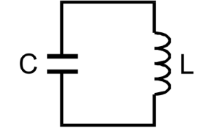
\includegraphics{content/UngedaempfterSchwingkreis.png}
  \caption{Schaltskizze eines ungedämpften Schwingkreises}
  \label{fig:ugsk}
\end{figure}



\subsection{Der reale Schwingkreis}

Der Unterschied zwischen idealem und realem Schwingkreis liegt darin, dass bei einem realen 
Schwingkreis ein ohmscher Widerstand eingebaut ist. Somit verliert der Schwingkreis über jede 
Periode hinweg Energie in Form von Joulscher Wärme. Diese Schaltung wird als gedämpfter 
Schwingkreis bezeichnet.

\begin{figure}[H]
  \centering
  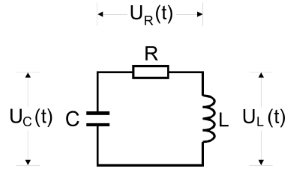
\includegraphics{content/GedaempfterSchwingkreis.png}
  \caption{Schaltskizze eines gedämpften Schwingkreises}
  \label{fig:gsk}
\end{figure}

Wie der Abbildung  entnommen werden kann, bildet der RCL-Schwingkreis eine Masche. Nach
dem zweiten Kirchhoffschen Gesetz ist die Summe aller Spannungen in einer geschlossenen Masche 
gleich null. Somit ergibt sich für den RCL-Kreis die Gleichung
\begin{equation}
    U_R(t)+U_C(t)+U_L(t) = 0.
    \label{eq:dgl}
\end{equation}
Dabei gelten für die Spannungen die Beziehungen
\begin{align*}
    U_R(t) = R I(t) \\ 
    U_C(t) = \frac{Q(t)}{C} \\ 
    U_L(t) = L \frac{\mathrm{d}I}{\mathrm{d}t},
\end{align*}
\noindent
wobei für die Stromstärke 
\begin{equation}
    I(t) = \frac{\mathrm{d}Q(t)}{\mathrm{d}t}
\end{equation}
\noindent
gelten soll. Mithilfe dieser Zusammenhänge ergibt sich aus \ref{eq:dgl} die lineare 
Differentialgleichung zweiter Ordnung
\begin{equation}
    \ddot{I}(t) + \frac{R}{L}\dot{I}(t) + \frac{1}{RC}I(t) = 0,
\end{equation}
\noindent
welche sich mit Hilfe des Ansatzes
\begin{equation}
    I(t) = U e^{iwt}
\end{equation}
\noindent 
lösen lässt. Durch Einsetzen des Ansatzes ergibt sich schließlich die charakteristische Gleichung
\begin{equation}
    -w^2 + i\frac{R}{L}w+\frac{1}{LC} = 0.
\end{equation}
\noindent
Mit den beiden Kreisfrequenzen $w_1$ und $w_2$ 
\begin{equation}
    w_{1,2} = i \frac{R}{2L} \pm \sqrt{\frac{1}{LC}-\frac{R^{2}}{4L^{2}}}
\end{equation}
\noindent
kann die allgemeine Lösung der Differentialgleichung 
\begin{equation}
    I(t) = U_1 e^{i w_1 t} + U_2 e^{i w_2 t},
    \label{eq:lsg}
\end{equation}
\noindent
wobei $U_1$ und $U_2$ komplexe Koeffizienten darstellen, bestimmt werden. Wird nun die 
Darstellung
\begin{align}
    \mu = \frac{R}{4\pi L} \nonumber \\
    \nu = \frac{1}{2\pi} \sqrt{\frac{1}{LC}-\frac{R^{2}}{4L^{2}}} \nonumber \\
\end{align}
\noindent
verwendet, lässt sich \ref{eq:lsg} zu
\begin{equation}
    I(t) = e^{-2\pi \mu t} \left( U_1 e^{i 2 \pi \nu t} + U_2 e^{-i 2 \pi \nu t} \right)
    \label{eq:Stromstaerke}
\end{equation}
\noindent
umschreiben. Dabei kann zwischen drei Fällen unterschieden werden, die nun vorgestellt 
werden sollen.








\subsubsection{Der Schwingfall}
Der erste Fall tritt dann ein, wenn $\frac{1}{LC} > \frac{R^{2}}{4L^{2}}$ gilt, was bedeutet,
dass $\nu_{1,2}$ zu imaginären Größen werden. Damit eine reelle Lösung zustande kommt, muss
zwischen $U_1$ und $U_2$ notwendigerweise die Beziehung $U_1 = \bar{U_2}$ gelten. Folglich lassen 
sie sich mithilfe der Euler-Formel in die Form
\begin{align*}
    U_1 = \frac{1}{2} A_0 e^{i \eta} \\
    U_2 = \frac{1}{2} A_0 e^{-i \eta}
\end{align*}
\noindent bringen. Somit kann die Gleichung \ref{eq:Stromstaerke} in
\begin{equation*}
    I(t) = A_0 e^{-2\pi \mu t} \cos{2\pi \nu t + \eta}
\end{equation*}
\noindent umgeformt werden. In diesem Fall liegt also eine gedämpfte harmonische Schwingung vor, 
dessen Amplitude mit fortlaufender Zeit exponentiell abnimmt. Die Schwingungsdauer kann
mit Hilfe des Zusammenhangs $T = \frac{1}{\nu}$ ermittelt werden. Für die allgemeine 
gedämpfte Schwingung ergibt sich 
\begin{equation}
    T = \frac{2\pi}{\sqrt{\frac{1}{LC}-\frac{R^{2}}{4L^{2}}}}, 
\end{equation}
\noindent wobei zusätzlich die Abnahmegeschwindigkeit der Amplitude durch den Wert 
\begin{equation}
    T_{ex} = \frac{1}{2\pi\mu} = \frac{2L}{R}
\end{equation}
\noindent beschrieben werden kann, welcher angibt, wann die Amplitude sich um den Faktor $e$
verkleinert hat.

\begin{figure}[H]
  \centering
  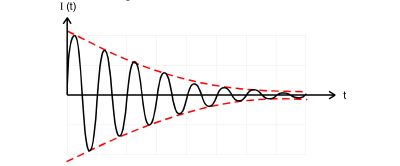
\includegraphics{content/VerlaufGedaempfteSchwingung.png}
  \caption{Zeitlicher Verlauf einer gedämpften Schwingung}
  \label{fig:gsk}
\end{figure}


\subsubsection{Der Kriechfall}

Der zweite Fall tritt ein, falls $\frac{1}{LC} \l \frac{R^{2}}{4L^{2}}$ gilt, was dazu führt, 
dass \nu selbst eine imaginäre Zahl darstellt. Damit enthält Gleichung \ref{eq:Stromstaerke}
lediglich reelle Exponentialfunktionen, was bedeutet, dass keine Schwingung ausgeführt wird, 
sondern die Amplitude - abhängig von den Werten $A_1$ und $A_2$ - entweder direkt und 
monoton gegen null geht oder zuerst ein Maximum erreicht (die sogenannte Überschwingung) 
und dann gegen null strebt. Diese Verläufe sind in Abbildung \ref{fig:fvs} dargestellt.


\subsubsection{Der aperiodische Grenzfall}

Der dritte und letzte Fall tritt ein, wenn $\frac{1}{LC} = \frac{R_{ap}}{4L^{2}}$ gilt, was dazu
führt, dass $\nu$ selbst null ergibt. Aus der Bedingung und Gleichung \ref{eq:Stromstaerke} ergibt
sich für den zeitlichen Verlauf der Stromstärke 
\begin{equation*}
    I(t) = A e^{-\frac{R}{2L}t}
\end{equation*}
\noindent wobei angemerkt werden soll, dass hierbei keine Überschwingung auftreten kann und 
das die Stromstärke hierbei noch schneller als beim Kriechfall gegen null strebt (siehe Abbildung \ref{fig:fvs}). 

\begin{figure}[H]
  \centering
  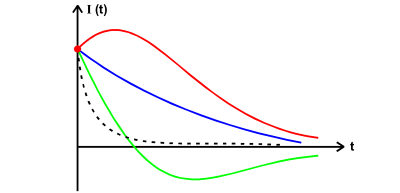
\includegraphics{content/faellevonschwingungen.png}
  \caption{Darstellung des Kriechfalls und des aperiodischen Grenzfalls (gestrichelte Kurve)}
  \label{fig:fvs}
\end{figure}









\subsection{Erzwungene Schwingungen}


\begin{figure}[H]
  \centering
  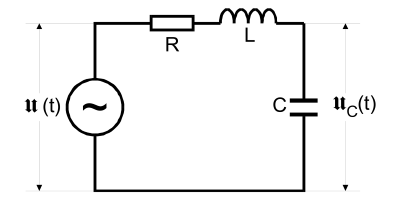
\includegraphics{content/ErzwungenerSchwingkreis.png}
  \caption{Schaltskizze eines erzwungenen RLC-Schwingkreises}
  \label{fig:esk}
\end{figure}



Durch den Einbau einer Wechselstromquelle können am RCL-Kreis auch erzwungene Schwingungen 
betrachtet werden. Der schematische Aufbau für die Schaltung lässt sich der Abbildung \ref{fig:esk}
entnehmen. Für den von außen mit der Wechselspannung $U(t) = U_0 e^{i\omega t}$ angetriebenen 
RCL-Kreis, geht Gleichung \ref{eq:dgl} in 
\begin{equation}
    L \frac{\mathrm{d}I}{\mathrm{d}t} + RI + \frac{Q}{C} = U_0 e^{}
\end{equation}
\noindent über. Weiterhin lässt sich diese auf die Form
\begin{equation}
    LC \frac{\mathrm{d}^{2}U_C}{\mathrm{d}t^{2}} + RC \frac{\mathrm{d}U_C}{\mathrm{d}t} + U_C = U_0 e^{i\omega t}
\end{equation}
\noindent bringen. Durch den Ansatz $U_C(\omega,t) = \tilde{U}(\omega) e^{i\omega t}$ ($\tilde{U}(\omega)$ ist 
eine komplexe Zahl) ergibt sich 
für die frequenzabhängigen Amplitude 
\begin{equation}
    \tilde{U}_C(\omega) = \frac{U_0(1-LC\omega^{2}-i\omega RC)}{(1-LC \omega^{2})^{2} + \omega^{2}R^{2}C{2} }
\end{equation}
beziehungsweise für dessen Betrag
\begin{equation}
    |\tilde{U}_C(\omega)| = U_C(\omega)= \frac{U_0}{\sqrt{(1-LC\omega)^{2})^{2}+\omega^{2}R^{2}C^{2}}}.
\end{equation}
Diese wird auch als Resonanzkurve bezeichnet. Zusätzlich ergibt sich als Zusammenhang
zwischen Phasenverschiebung und Frequenz $\omega$
\begin{equation}
    \phi(\omega) = \arctan{\frac{-\omega RC}{1-LC \omega^{2}}}.
\end{equation}
\noindent
Für $\omega \rightarrow \infty$ gilt
$U_C \rightarrow 0$ und für $\omega \rightarrow 0$ gilt $U_C \rightarrow U_0$. Falls die 
sogenannte Resonanzfrequenz 
\begin{equation}
    \omega_{res} = \sqrt{\frac{1}{LC} - \frac{R^{2}}{2L^{2}}}
\end{equation}
\noindent 
sich der Eigenfrequenz 
\begin{equation}
    \omega_0 = \sqrt{\frac{1}{LC}}
\end{equation}
nähert, kann die Kondensatorspannung $U_C$ aber auch größter als die anliegende Generatorspannung
$U_0$ sein. Im Fall der schwachen Dämpfung
\begin{equation*}
    \frac{R^{2}}{2L^{2}} \ll \frac{1}{LC}
\end{equation*}
\noindent 
überschreitet die Kondensatorspannung die Generatorspannung, wobei 
\begin{equation}
    U_{C,max} = \frac{1}{\omega_0 RC} U_0 
\end{equation}
\noindent
den Zusammenhang darstellt. Falls $R \rightarrow 0$ strebt, geht $U_C \rightarrow \infty$. Dies 
wird als Resonanzkatastrophe bezeichnet. Die Güte des Schwingkreises ergibt sich durch
\begin{equation}
    q = \frac{1}{\omega_0 RC}.
\end{equation}
\noindent
Weiterhin wird die Breite der Resonanzkurve durch die Differenz der beiden Frequenzen 
\begin{equation}
    \omega_+ - \omega_- \approx \frac{R}{L}
\end{equation}
angegeben, an denen die Kondensatorspannung, unter der Bedingung 
$\frac{R^{2}}{L{2}} \ll \omega_0^{2}$, auf das $\frac{1}{\sqrt{2}}$-fache
ihres Maximalwerts abgefallen ist.  

Für $\frac{R^{2}}{2L^{2}} \gg \frac{1}{LC}$ liegt eine starke Dämpfung vor. Bei $\omega_0$ liegt
eine Phasenverschiebung von $\phi = -\frac{\pi}{2}$ vor. Die Frequenzen $\omega_1$ (bei $\phi = \frac{\pi}{4}$) und
$\omega_2$ (bei $\phi = \frac{3}{4}\pi$) lassen sich mit 
\begin{equation}
    \omega_{1,2} = \pm \frac{R}{2L} + \sqrt{\frac{R^{2}}{4L^{2}}+\frac{1}{LC}}
\end{equation}
\noindent berechnen.

\section{Durchführung}
\label{sec:Durchführung}

\section{Auswertung}
\label{sec:Auswertung}

\begin{figure}
  \centering
  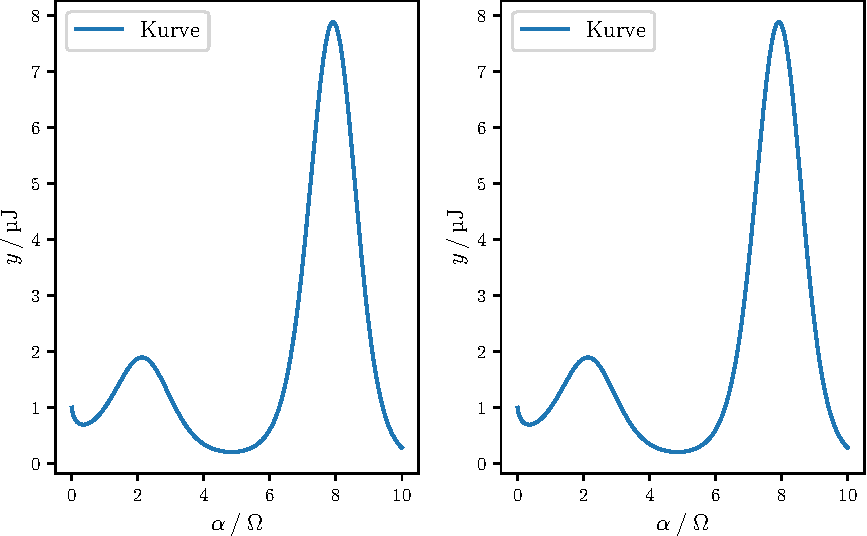
\includegraphics{plot.pdf}
  \caption{Plot.}
  \label{fig:plot}
\end{figure}


Siehe \autoref{fig:plot}!

\section{Diskussion}
\label{sec:Diskussion}
Das vom Oszilloskopen aufgenommene Bild \ref{fig:a1}
entspricht der erwarteten Form einer gedämpften Schwingung (siehe \ref{fig:gsk})
Allerdings fällt auf, dass die Abklingdauer viel zu groß ist.
Würde direkt der Betrag der Steigung als Abklingdauer angenommen werden,
so würde sich für $R_{eff}$ ein wahrscheinlicherer Wert von
\begin{equation*}
    R_{eff}=(678\pm19)\,\si{\ohm}
\end{equation*}
\noindent ergeben. Dieser Wert würde dem tatsächlichen Widerstandwert
von $R=(30,3\pm0,1)\,\si{\ohm} + 600\,\si{\ohm}$ eher entsprechen als der
in \ref{sec:dae} errechnete Wert.
-Problem mit Inversem erklären?
-Probelm, dass Innenwiderstand vielleicht nicht dem
unseres Gerätes entspricht


Bei der Messung der Phasenverschiebung wurden nicht
genug Werte aufgenommen um den nach Gleichung (REFERENZ)
erwarteten Verlauf eines Arcustangens zu erkennen.
Außerdem stechen einige Werte, wie der dritte Messwert
in Abbildung \ref{fig:c} ungewöhnlich hervor, was
wohl auf ein falsches Ablesen der Größen $a$ oder
$b$ zurückzuführen ist. Bei der Bestimmung
von $\omega_1$ und $\omega_2$ sind Ungenauigkeiten
dadurch entstanden, dass jeweils der Wert abgelesen wurde,
welcher am nähsten am gesuchten Vielfachen von $\pi$
liegt. Doch diese Ungenauigkeiten können nicht erklären,
warum vro allem $\omega_2=283\,\si{\kilo\hertz}$ so stark vom errechneten Wert
$\omega_2=(394\pm0,9)\,\si{\kilo\hertz}$ abweicht.
(VERWEIS AUF PROBLEM MIT INNENWIDERSTAND?)
\section{Anhang}
\begin{figure}
    \centering
    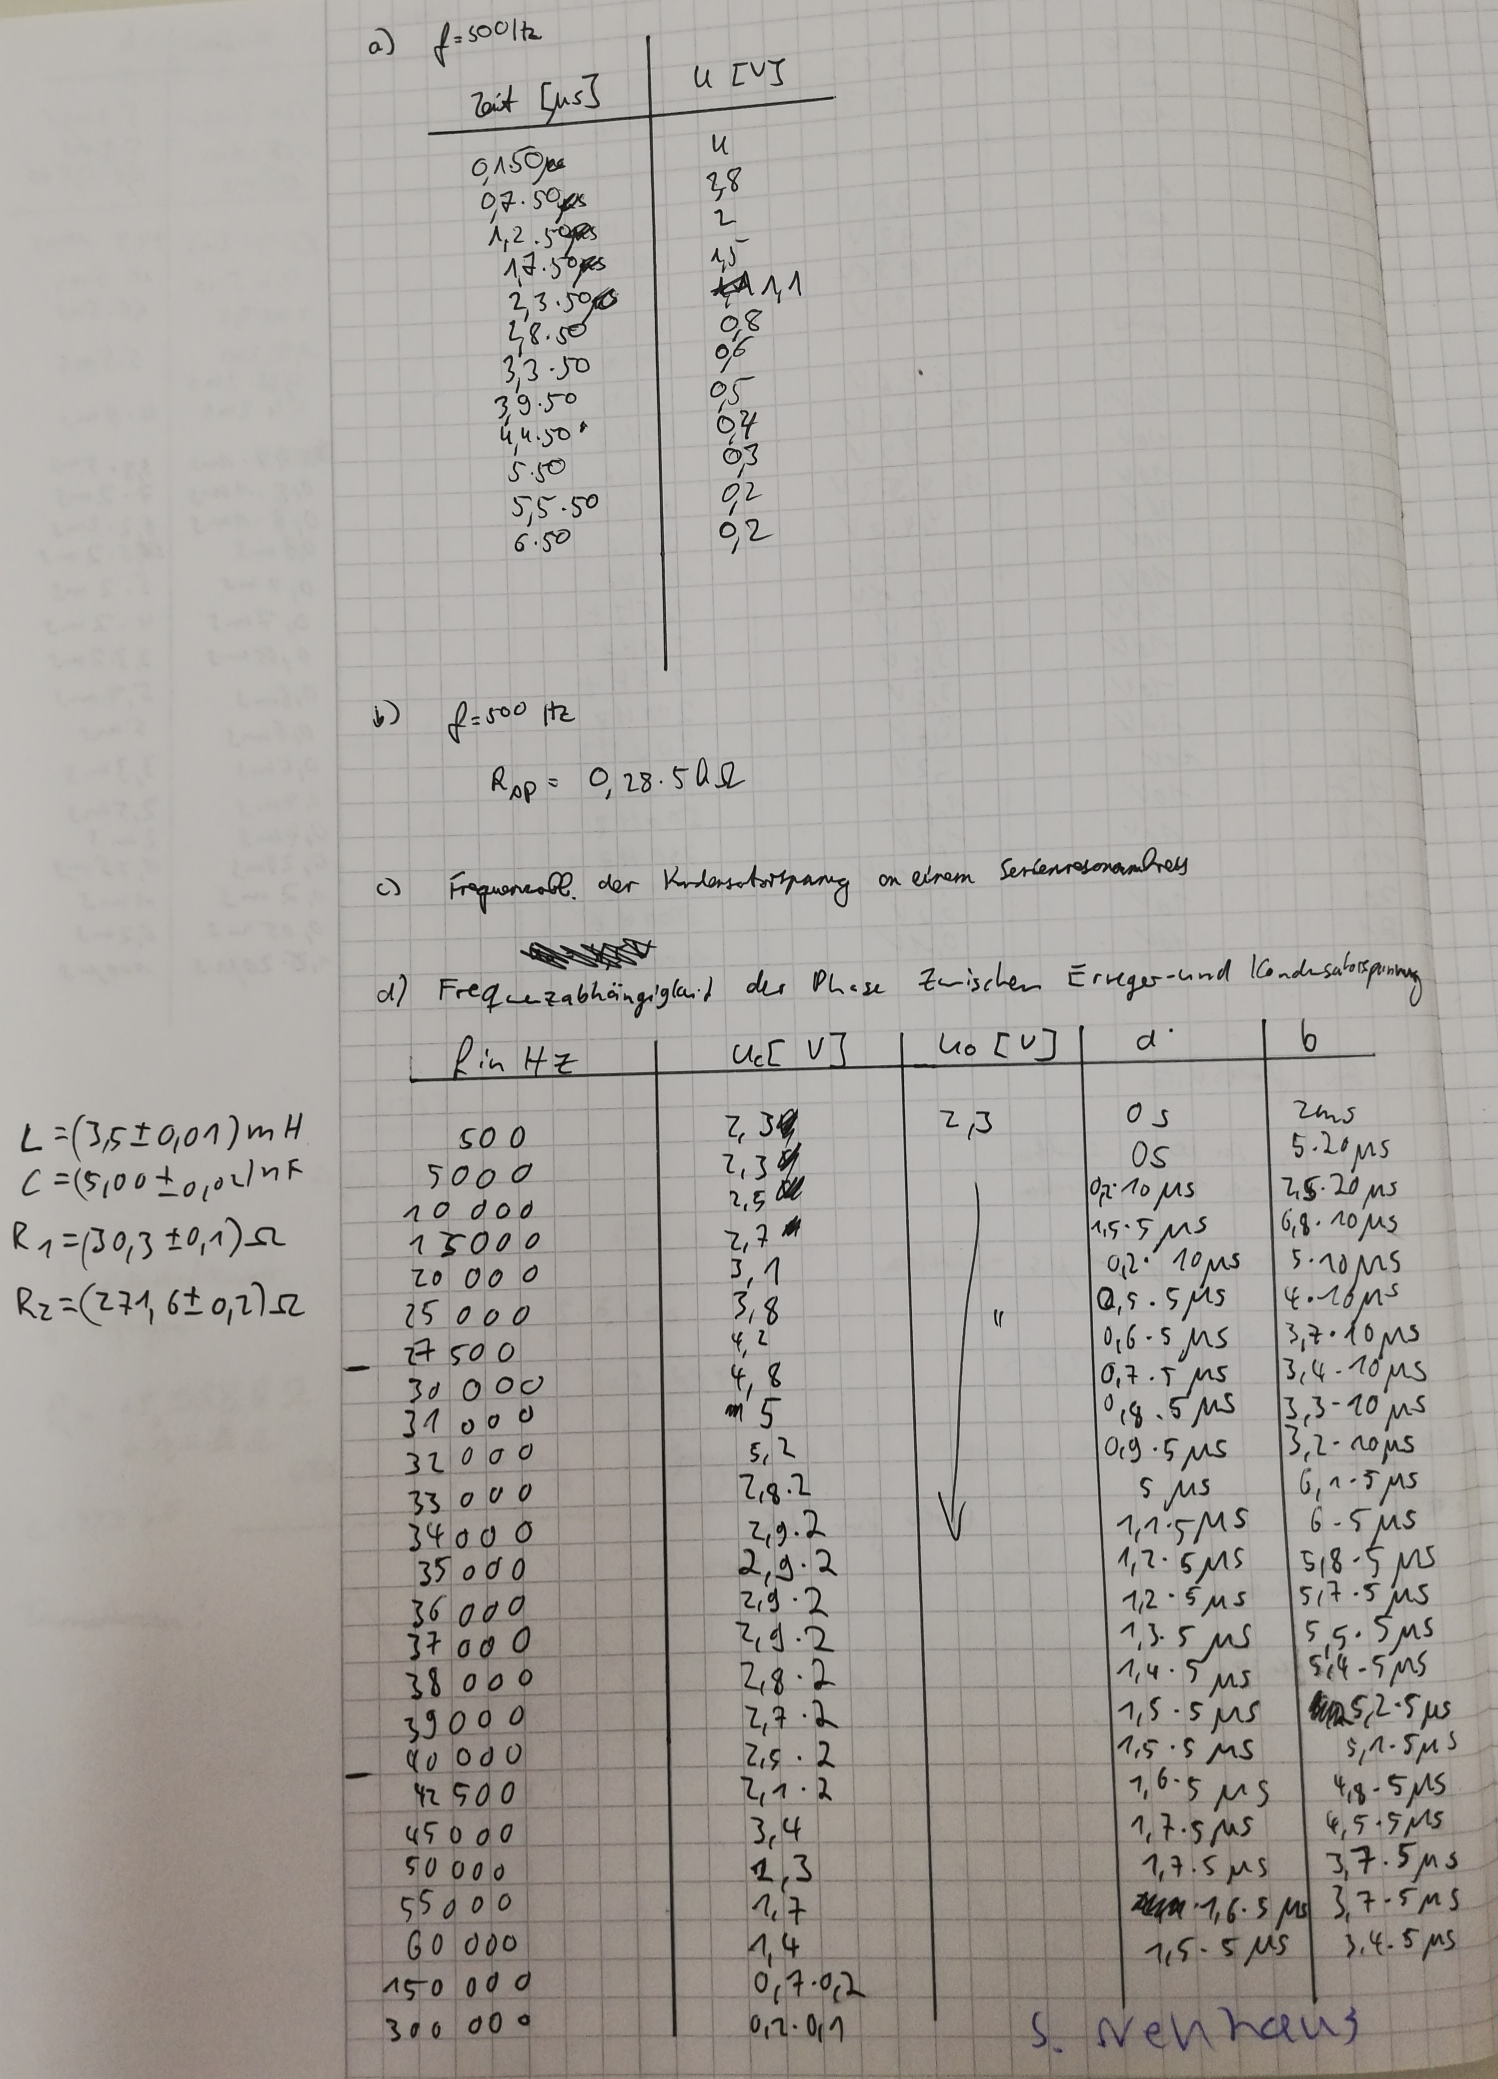
\includegraphics[width=15cm]{content/Anhang.jpg}
\end{figure}
\nocite{*}
\printbibliography{}

\end{document}
